In this Section, we report on our analysis of the dataset we built, focusing on the most interesting findings. The interested reader will find our data exploration and extended analysis in the companion notebook.

\subsection{Duration of the Battles}

We observe that the duration of the battles over the last millennium increased almost monotonically. In fact, we can see in Figure \ref{fig:durThByCent} that the average duration of a battle has never been higher than nowadays. Notice that the average duration of a battle was almost 34 days during the XX$^{th}$ century while it is currently of 64 days in the XXI$^{st}$ century.

 \begin{figure}[h]
	\centering	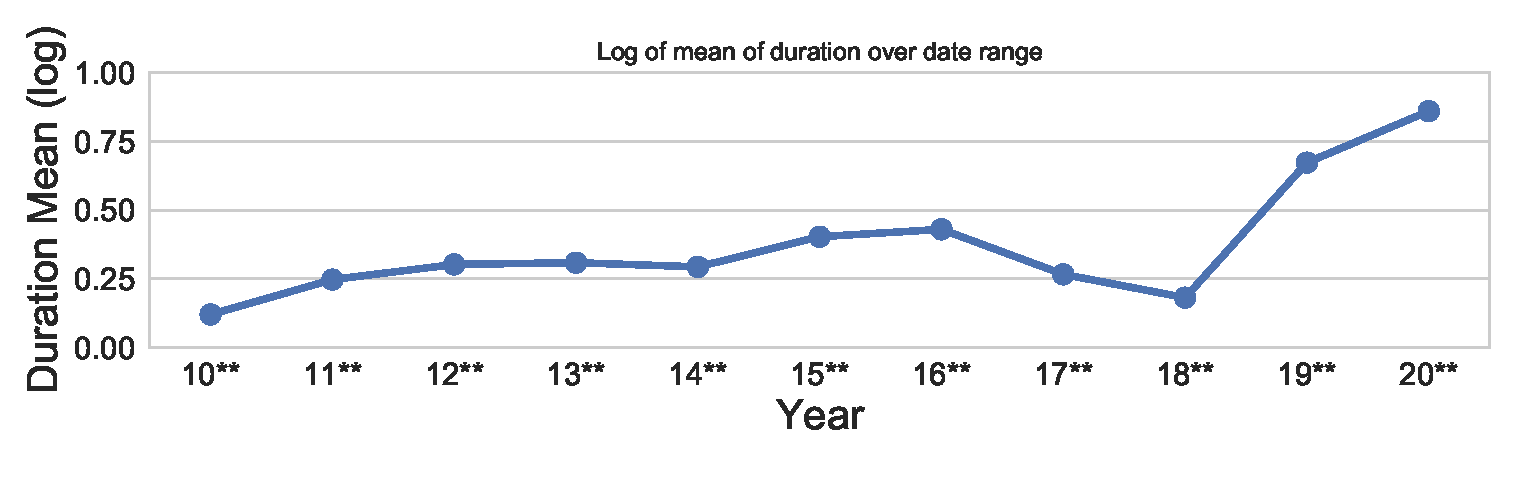
\includegraphics[width=\linewidth]{figures/durThByCent}
	\caption{Mean of the duration of battles in the last thousand years by century on a logarithmic scale.}\label{fig:durThByCent}
	\centering
\end{figure}

\subsection{Evolution of the Casualties}

In Figure \ref{fig:casuPerCent}, we notice that the percentage of soldiers engaged in a battle that are wounded, killed, captured or that disappeared decreases throughout the years. We observe that, following the same trend as shown in Figure \ref{fig:durThByCent} for the battle's duration, the percentage of casualties decreased before increasing in the XX$^{th}$ century. We can infer that in both cases this is due to the world wars because they contain numerous battles which made countless casualties, notably because of technology advances such as aerial forces or gaz attacks.
 \begin{figure}[h]
	\centering	\includegraphics[width=\linewidth]{figures/casuPerCent}
	\caption{Mean of the percentage of casualties in the soldiers.}\label{fig:casuPerCent}
	\centering
\end{figure}

\subsection{Indecisiveness of the Battles}

We observe, in Figure \ref{fig:IndecBattles}, that battles tend to be more indecisive nowadays than they were in the past. In fact, the fraction of indecisive battle within one century is increasing slowly since year 1200 at a much higher rate over the last two centuries. This can be explained by two factors: the first being that battles in the further past were most likely reported by the winner who would, and with less accuracy and objectiveness as they are now. The second explanation lies in operational theaters (like cities) and tactics enabled by modern weaponry such as long range weapons. Ultimately, longer distance between the combatants and modern combat vehicles greatly enhanced the ability to retreat.

 \begin{figure}[h]
	\centering	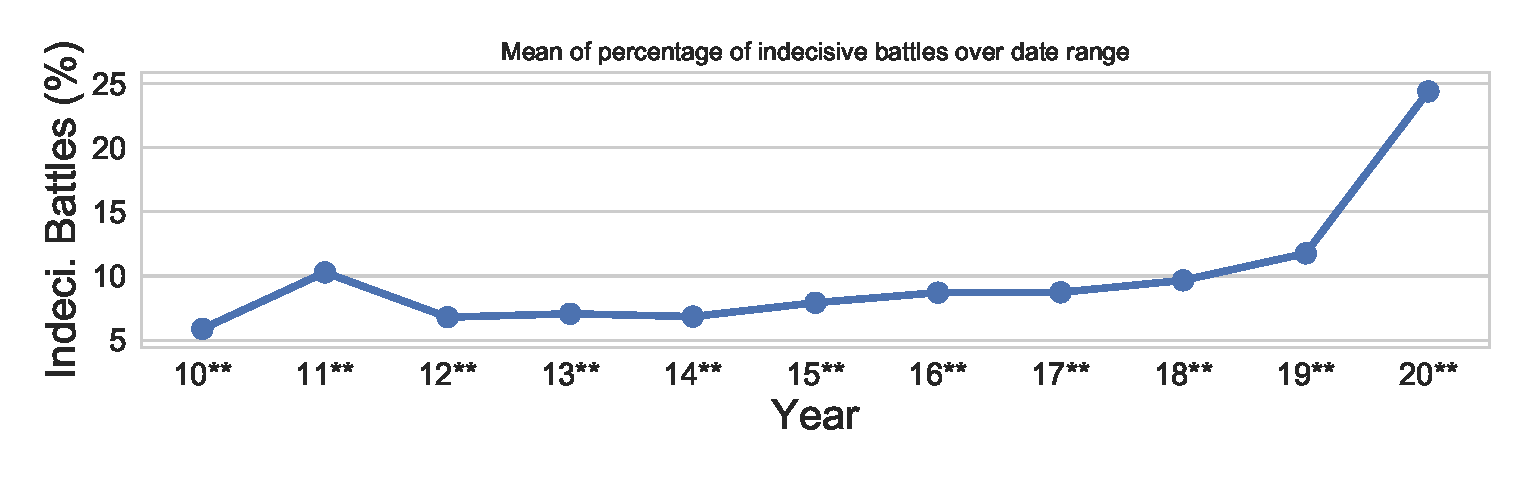
\includegraphics[width=\linewidth]{figures/indThByCent}
	\caption{Mean of the number of indecisive battles over the last thousand years by century on a logarithmic scale.}\label{fig:IndecBattles}
	\centering
\end{figure}

From Figures \ref{fig:durThByCent}, \ref{fig:casuPerCent} and \ref{fig:IndecBattles}, we conclude that battles are longer, make less casualties and are more indecisive over the years. This supports the fact that nowadays the battle's purpose is not only to invade another territory by beating the other combatant. In fact, modern battles seem to be more complex in the sense that they often serve a higher strategic or even political goal and have their result studied in many different axis.

\subsection{Outcome of the battles}

We continue our analysis by studying the advantage provided to a combatant that has fewer of casualties, larger strengths  and  lower casualties to strength ratio. We compute the percentage of battles won by a combatant that had at least one of these advantages, grouped by three different victory types: \textit{tactical}, \textit{strategic},  \textit{decisive}. The \textit{tactical} level is the lower one in the military level of planning\cite{military_planning}, therefore involving narrower scope decisions and shorter-term consequences. On the other end, the \textit{strategic} level is the highest one, involving longer-term
consequences.

We first observe that an advantage in strength only is not sufficient to increase one's chances to win a battle, as this would completely disregard other tactical advantage of the opponent. On the other hand, the a-posteriori advantage in the casualties (both in ratio and absolute value) is much more significant, as it is present in around 75\% of the victories for all but strategic ones. Very interestingly, we observe that for this victory type, an advantage in absolute casualties has much less effect on the outcome (in fact, it looks like it is the opposite), and a little less effect in the ratio advantage. This would typically generalize the mentioned case of the Battle for Stalingrad, where the Nazi Germany strategy was not able to provide victory even though it was tactically superior. Figure \ref{fig:victoryAdvantage} illustrates these observations.

 \begin{figure}[h]
	\centering	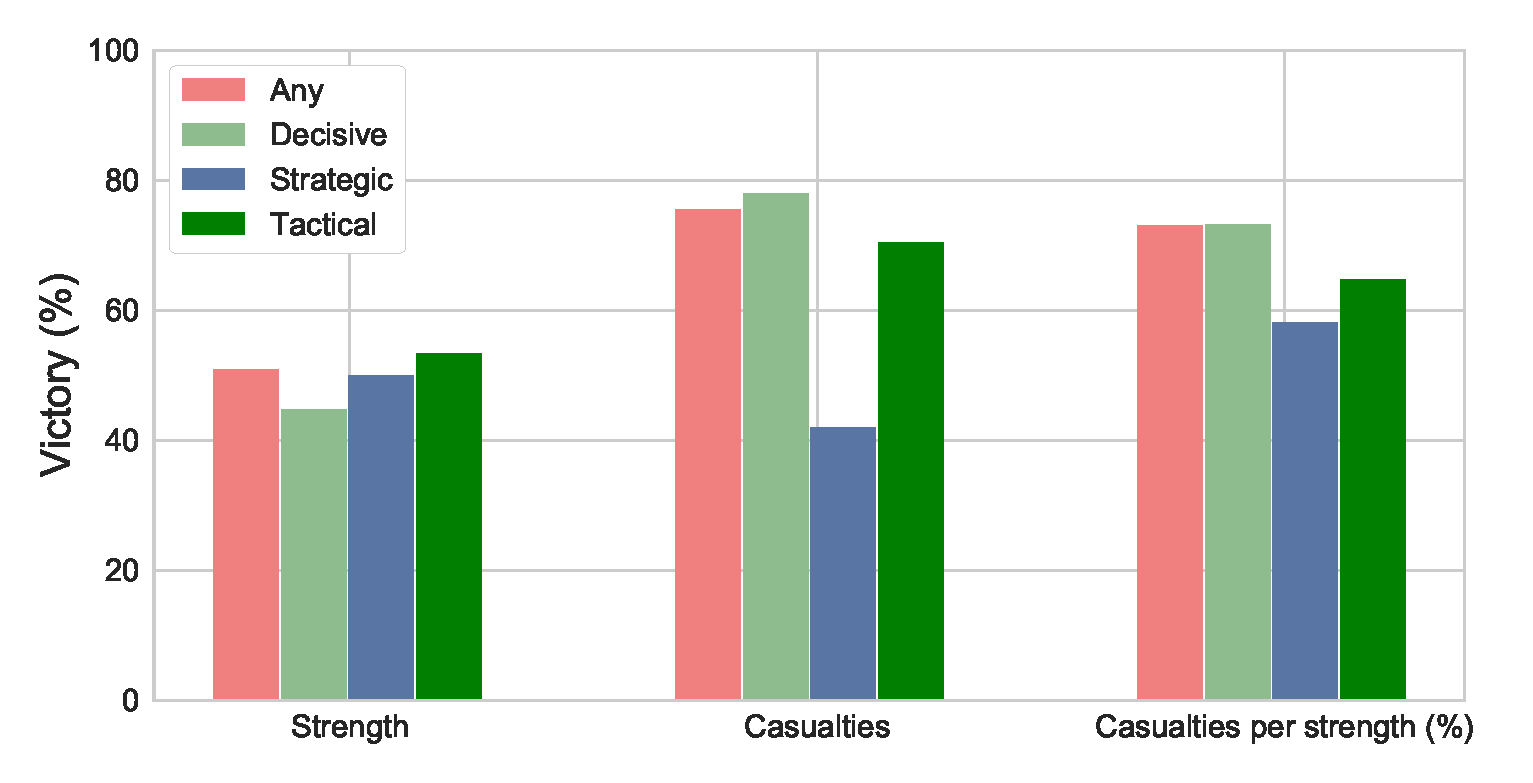
\includegraphics[width=\linewidth]{figures/VictoryAdvantage}
	\caption{Victory percentage with advantage in either strength, casualties or casualty ratio.}\label{fig:victoryAdvantage}
	\centering
\end{figure}

\subsection{Years of Battles per Countries}
In Figure \ref{fig:FightingDurationRanking}, we observe that among all countries in our dataset, France is the one that fought the most. Nevertheless, the United States, which are a major actor in the international history of battles, were only created in 1776 when they proclaimed their independence. Thus, it is interesting to do the same ranking starting from this year. 
 \begin{figure}[h]
 	\centering
 	\begin{subfigure}[b]{0.475\linewidth}
 		\centering
 		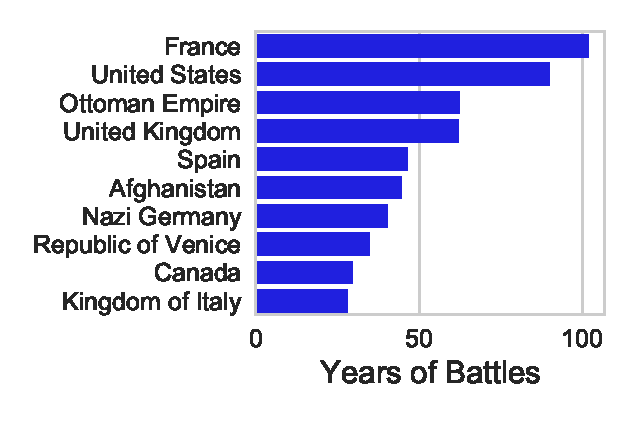
\includegraphics[width=\linewidth]{figures/YearsFightingRanking.eps}
 		\caption[]%
 		{{\small 1000 --- 1700}}    
 		\label{fig:FightingDurationRankingOld}
 	\end{subfigure}
 	\begin{subfigure}[b]{0.475\linewidth}  
 		\centering 
 		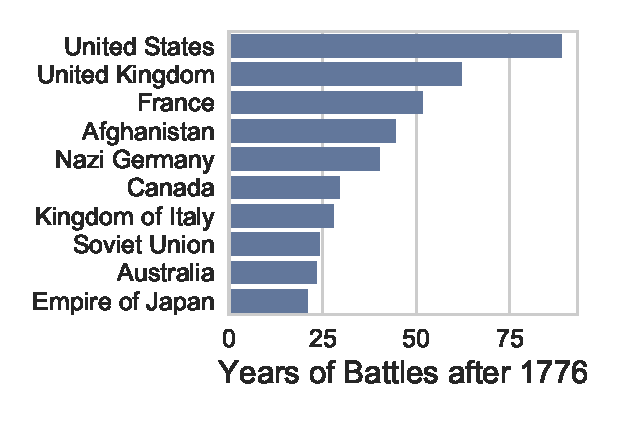
\includegraphics[width=\linewidth]{figures/YearsFightingRankingModern}
 		\caption[]%
 		{{\small 1701 --- 1900}}    
 		\label{fig:FightingDurationRankingModern}
 	\end{subfigure}
 	\vskip0.2\baselineskip
	\caption{Cumulated duration of battles engagement per country. From 100 in (a) and from 1776 and the United States independence in (b).} 
 	\label{fig:FightingDurationRanking}
 \end{figure}
 
 These results tend to support the common belief that the United States are always in war. In fact, as we observe in Figure \ref{fig:USAFightingTimeline}, they were engaged in a at least one battle per year for more than 150 years in 242 years of existence.
 \begin{figure}[h]
 	\centering	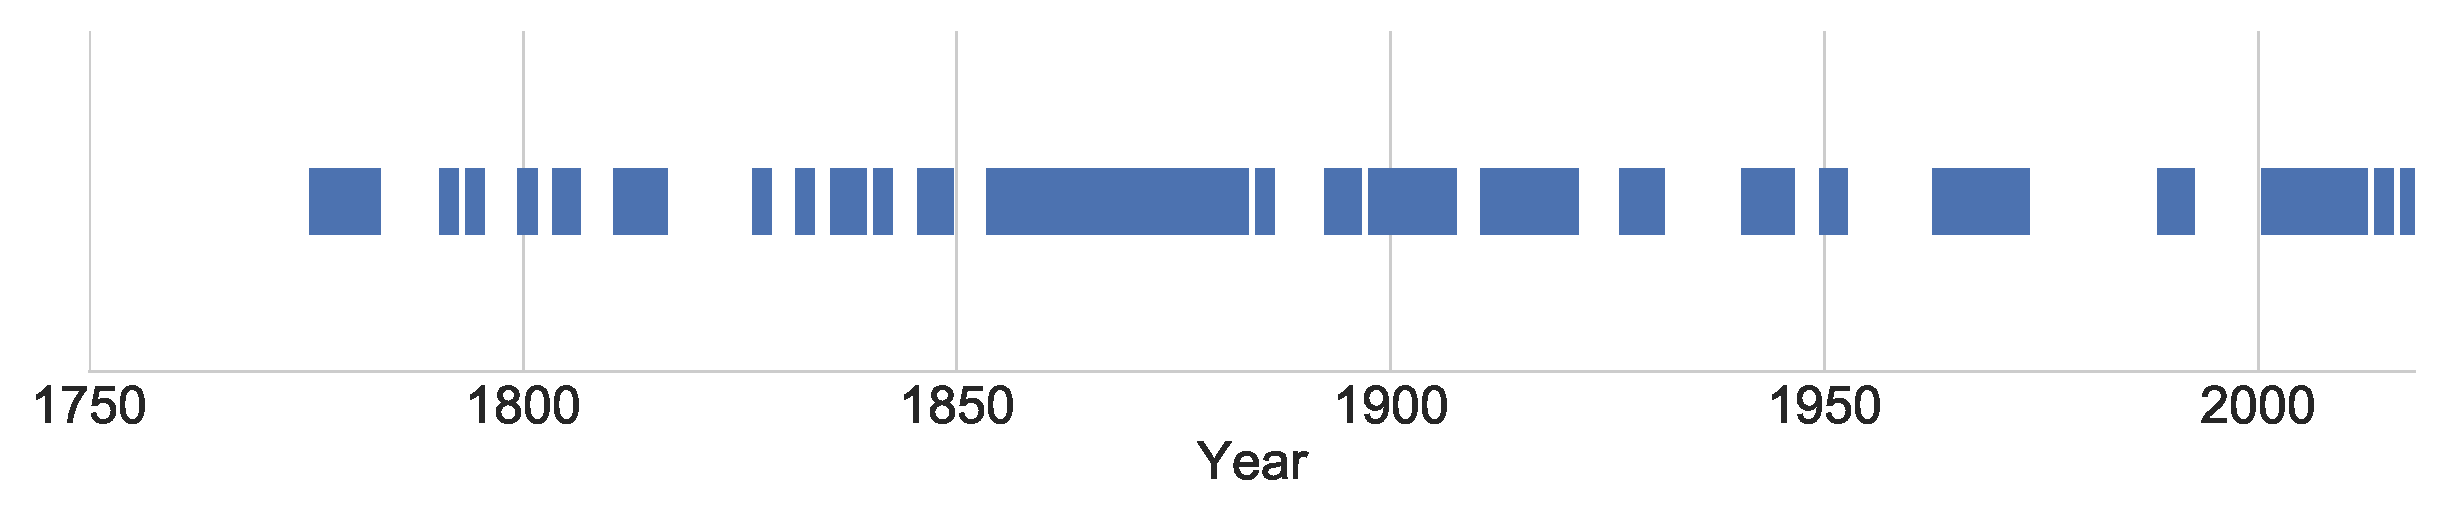
\includegraphics[width=\linewidth]{figures/USAFighting}
 	\caption{Timeline of the USA engagement in battles.}\label{fig:USAFightingTimeline}
 	\centering
 \end{figure}

